%Version 3.1 December 2024 — Springer Nature LaTeX template (sn-jnl)
\documentclass[pdflatex,sn-mathphys-num]{sn-jnl}% Math and Physical Sciences Numbered Reference Style

%%%% Standard Packages
\usepackage{graphicx}%
\usepackage{multirow}%
\usepackage{amsmath,amssymb,amsfonts}%
\usepackage{amsthm}%
\usepackage{mathrsfs}%
\usepackage[title]{appendix}%
\usepackage{xcolor}%
\usepackage{textcomp}%
\usepackage{manyfoot}%
\usepackage{booktabs}%
\usepackage{algorithm}%
\usepackage{algorithmicx}%
\usepackage{algpseudocode}%
\usepackage{listings}%

\theoremstyle{thmstyleone}%
\newtheorem{theorem}{Theorem}%
\newtheorem{proposition}[theorem]{Proposition}%

\theoremstyle{thmstyletwo}%
\newtheorem{example}{Example}%
\newtheorem{remark}{Remark}%

\theoremstyle{thmstylethree}%
\newtheorem{definition}{Definition}%

\raggedbottom

\begin{document}

\title[Anomaly Detection on Smart Home Energy Data]{Anomaly Detection on Smart Home Energy Data: An Exploratory Analysis and Comparative Machine-Learning Study Using the HomeC Dataset}

\author*[1]{\fnm{First} \sur{Author}}\email{author@fpt.edu.vn}

\author[1]{\fnm{Second} \sur{Author}}\email{author2@fpt.edu.vn}
\equalcont{These authors contributed equally to this work.}

\author[1]{\fnm{Third} \sur{Author}}\email{author3@fpt.edu.vn}
\equalcont{These authors contributed equally to this work.}

\affil*[1]{\orgdiv{Department of Artificial Intelligence and Data Science}, \orgname{FPT University}, \orgaddress{\city{Ho Chi Minh City}, \country{Vietnam}}}

%%==================================%%
%% Abstract                          %%
%%==================================%%

\abstract{Smart home metering systems generate high-frequency, appliance-level energy data that can be mined to detect abnormal consumption, which in turn signals equipment faults, inefficiency, or unusual occupant behaviour. This study investigates anomaly detection on the publicly available HomeC dataset (Smart Home Dataset with Weather Information), comprising 503{,}910 minute-level observations spanning January to mid-December 2016. Because the dataset contains no ground-truth anomaly labels, we construct a statistical proxy label using a $\mu + 3\sigma$ threshold on whole-house consumption, yielding an anomaly rate of 2.46\%. We perform a full exploratory data analysis, engineer time- and appliance-based features, and benchmark five models---Logistic Regression, Random Forest, XGBoost, LightGBM, and Isolation Forest---under a leakage-controlled pipeline that applies standardisation and SMOTE only to the training partition. Random Forest achieved the strongest performance (F1 = 0.941, AUC = 0.9996), followed closely by XGBoost (F1 = 0.933). The analysis further shows that appliance usage---particularly heating circuits, which account for roughly 56\% of metered appliance energy---dominates consumption variability, whereas weather variables correlate meaningfully with solar generation ($r \approx 0.36$ for temperature) but only weakly with raw household demand. The results are delivered through an interactive dashboard that surfaces key performance indicators, anomaly alerts, and energy-saving recommendations.}

\keywords{anomaly detection, smart home energy, exploratory data analysis, machine learning, time-series, ensemble methods}

\maketitle

%%==================================%%
\section{Introduction}\label{sec:intro}

The proliferation of smart home technologies has made continuous, fine-grained monitoring of household electricity consumption routine. Networked sensors and smart plugs produce large time-series datasets that, when analysed, can improve energy efficiency, reduce operating cost, and enrich home-automation logic. Within these data streams, abnormal consumption events are of particular interest: a sustained or sudden deviation from typical usage can indicate a malfunctioning appliance, inefficient operation, atypical occupant activity, or a faulty sensor. Left undetected, such patterns translate into higher energy bills, shortened equipment lifespan, and wasted resources.

Conventional monitoring relies on manual inspection and fixed thresholds, which scale poorly and struggle to capture context-dependent abnormality across many appliances. Data-driven methods offer a more flexible alternative by learning consumption structure directly from historical data and flagging departures from it. The HomeC dataset is well suited to this investigation because it combines appliance-level power measurements with concurrent weather observations, allowing both the internal drivers of consumption and the external influence of environmental conditions to be examined together.

This paper pursues three goals. First, it characterises household energy-consumption behaviour through exploratory data analysis. Second, it formulates anomaly detection as a supervised classification task via a transparent statistical proxy label and benchmarks several models against it. Third, it examines the relationship between weather and energy, distinguishing the drivers of consumption from those of on-site solar generation. The contributions are summarised as follows:

\begin{itemize}
\item A reproducible preprocessing and feature-engineering pipeline for the HomeC dataset, including a corrected reconstruction of the time axis.
\item A leakage-controlled comparative evaluation of five models, with Random Forest and XGBoost emerging as the strongest detectors.
\item An empirical account of which appliance and weather factors are associated with abnormal consumption, delivered through an interactive analytics dashboard.
\end{itemize}

%%==================================%%
\section{Problem Statement and Research Questions}\label{sec:problem}

\subsection{Problem Definition}
The objective is to identify abnormal electricity-consumption periods within a single smart home using data analytics and machine learning. This entails three coupled tasks: understanding consumption behaviour, characterising the relationships among appliance and weather variables, and building and evaluating models that distinguish normal from abnormal periods.

\subsection{Research Questions}
The study is organised around three research questions that build on one another. We begin by asking what factors are associated with abnormal energy consumption (RQ1): before any detector can be trusted, it is necessary to understand which appliance-related and weather-related variables drive unusual usage, since this understanding both guides feature selection and lends interpretability to the anomalies that are eventually flagged. Having established which signals matter, we then ask which model performs best on this dataset (RQ2), comparing several detectors under common, imbalance-aware metrics---F1 and AUC-ROC---to identify the most effective approach. Finally, because the dataset uniquely pairs energy readings with concurrent weather observations, we ask whether weather genuinely influences household energy consumption (RQ3), quantifying the association between environmental variables such as temperature, humidity, and wind speed and both household demand and on-site solar generation. Together these questions move from understanding the data, to modelling it, to interpreting the external conditions that shape it.

%%==================================%%
\section{Dataset and Data Understanding}\label{sec:data}

\subsection{Dataset Overview}
We use the Smart Home Dataset with Weather Information (HomeC), obtained from Kaggle. The dataset records minute-level measurements over the 2016 calendar year and pairs appliance-level power readings with weather observations. Its principal characteristics are listed in Table~\ref{tab:dataset}.

\begin{table}[h]
\caption{HomeC dataset characteristics}\label{tab:dataset}
\begin{tabular}{@{}ll@{}}
\toprule
Attribute & Value \\
\midrule
Number of rows & 503{,}910 \\
Number of columns (raw) & 32 \\
Time range & 2016-01-01 to 2016-12-15 ($\approx$ 349 days) \\
Sampling interval & 1 minute \\
Data type & Multivariate time-series \\
Domain & Smart home energy consumption \\
\botrule
\end{tabular}
\end{table}

The features fall into three groups: \emph{energy} variables (\texttt{use [kW]}, \texttt{gen [kW]}, \texttt{House overall [kW]}); \emph{appliance} circuits (e.g. Furnace, Home office, Fridge, Dishwasher, Microwave, Living room, Garage door, Barn, Well, Wine cellar, and Kitchen circuits); and \emph{weather} variables (temperature, humidity, visibility, pressure, wind speed, cloud cover, dew point, precipitation probability and intensity, and a categorical weather \texttt{summary}/\texttt{icon}).

\subsection{Time-Axis Reconstruction}
An initial inspection revealed that the raw Unix \texttt{time} column increments by one second per row rather than one minute as the dataset description implies. Converting that column naively compresses all 503{,}910 records into roughly six days. Because every downstream time-based feature (hour, day-of-week, month, season) depends on a correct time axis, we reconstructed the index using a regular one-minute frequency over the full record count. This restores the true $\approx$ 349-day span and gives the seasonal and weekly features genuine variation, which is essential for both the exploratory analysis and the model features.

\subsection{Data Cleaning}
No missing values were detected across any feature, so no imputation was required. No duplicate rows were found. Two redundant columns (\texttt{House overall [kW]} and \texttt{Solar [kW]}), which duplicate information already present in \texttt{use [kW]} and \texttt{gen [kW]}, were removed to reduce multicollinearity. An interquartile-range scan identified roughly 34{,}000 extreme observations; these were deliberately retained, since in an anomaly-detection context extreme values are more likely to represent genuine abnormal behaviour than measurement error.

%%==================================%%
\section{Exploratory Data Analysis}\label{sec:eda}

This section answers RQ1 and RQ3 through visual and statistical analysis of the cleaned, full-year data.

\subsection{Consumption Over Time}
Figure~\ref{fig:timeseries} shows daily-aggregated household consumption across 2016. Usage fluctuates substantially, with several pronounced spikes that stand out as candidate anomalies. The series also exhibits seasonal structure that only becomes visible once the time axis is correctly reconstructed.

\begin{figure}[h]
\centering

\includegraphics[width=\textwidth]{figs/chart1_timeseries.png}
\caption{Household energy consumption over the full 2016 observation period.}\label{fig:timeseries}
\end{figure}

\subsection{Distribution of Consumption}
The distribution of minute-level consumption is strongly right-skewed (Figure~\ref{fig:hist}): most observations sit at low power levels, while high-consumption events are comparatively rare. The boxplot in Figure~\ref{fig:box} confirms a long upper tail with many points beyond the whiskers. This rarity of high-consumption events is precisely the regime in which anomaly-detection methods are appropriate, and it motivates the use of imbalance-aware evaluation metrics in Section~\ref{sec:eval}.

\begin{figure}[h]
\centering

\includegraphics[width=0.85\textwidth]{figs/chart2_histogram.png}
\caption{Distribution of minute-level household energy consumption.}\label{fig:hist}
\end{figure}

\begin{figure}[h]
\centering

\includegraphics[width=0.7\textwidth]{figs/chart3_boxplot.png}
\caption{Boxplot of energy consumption with the anomaly threshold indicated.}\label{fig:box}
\end{figure}

\subsection{Top Energy-Consuming Appliances (RQ1)}
Aggregating energy by appliance circuit over the full year (Figure~\ref{fig:top5}, Table~\ref{tab:top5}) shows a highly concentrated consumption profile. The heating circuits (Furnace 1 and 2, grouped) alone account for approximately 56\% of all metered appliance energy, far ahead of the Home office, Fridge, Barn, and Wine cellar circuits. This concentration identifies heating as the primary target for both anomaly monitoring and energy-saving recommendations.

\begin{figure}[t]
\centering
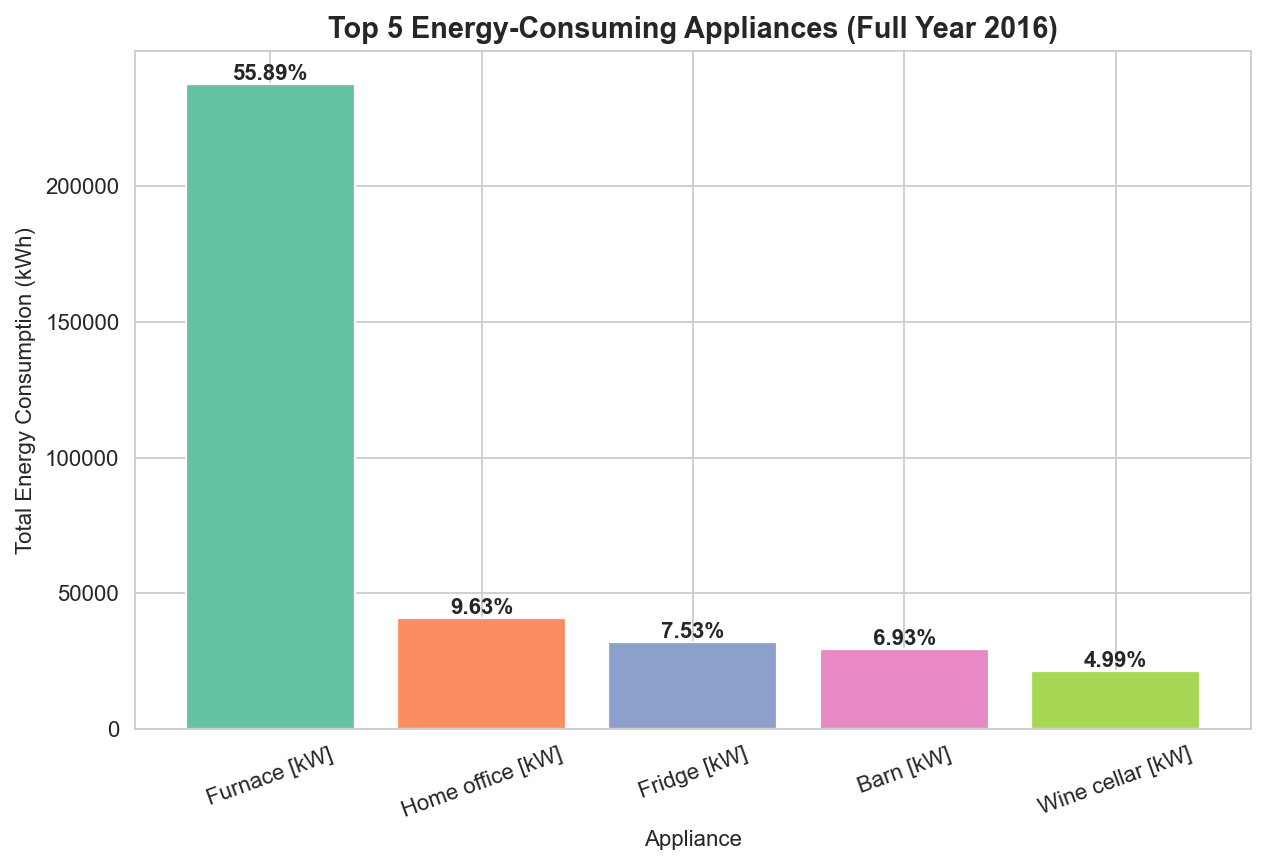
\includegraphics[width=0.85\textwidth]{figs/chart6_top5_appliances_bar.png}
\caption{Top-five energy-consuming appliance circuits over 2016.}\label{fig:top5}
\end{figure}

\begin{table}[t]
\caption{Top-five appliance circuits by total energy (full-year, grouped circuits)}\label{tab:top5}
\begin{tabular}{@{}lrrr@{}}
\toprule
Appliance & Total (kWh) & Share (\%) & Peak hour \\
\midrule
Furnace (1+2) & 237{,}835 & 55.89 & 05:00 \\
Home office   & 40{,}961  & 9.63  & 21:00 \\
Fridge        & 32{,}027  & 7.53  & 20:00 \\
Barn          & 29{,}494  & 6.93  & 16:00 \\
Wine cellar   & 21{,}233  & 4.99  & 17:00 \\
\botrule
\end{tabular}
\footnotetext{Shares are computed over total metered appliance energy. The peak hour is the hour of day with the highest mean consumption for that circuit.}
\end{table}

\subsection{Correlation Structure and Weather (RQ3)}
The correlation heatmap (Figure~\ref{fig:heatmap}) and the weather scatter analysis (Figure~\ref{fig:weather}) together address RQ3. Two findings stand out. First, on-site solar generation (\texttt{gen [kW]}) is moderately and positively correlated with temperature ($r \approx 0.36$), apparent temperature ($r \approx 0.36$), and dew point ($r \approx 0.29$), and weakly negatively correlated with wind speed ($r \approx -0.15$)---consistent with photovoltaic output rising on warmer, clearer, calmer days. Second, raw household demand (\texttt{use [kW]}) shows only weak correlation with any single weather variable ($|r| < 0.1$ throughout). At one-minute resolution, which appliances happen to be switched on explains far more of the variance in demand than outdoor conditions do. The practical implication is that weather is a useful predictor for generation, but appliance-level behaviour remains the dominant driver of consumption anomalies---supporting the feature choices made for modelling.

\begin{figure}[t]
\centering

\includegraphics[width=0.95\textwidth]{figs/chart4_heatmap.png}
\caption{Correlation heatmap across energy, top appliances, and weather variables.}\label{fig:heatmap}
\end{figure}

\begin{figure}[t]
\centering
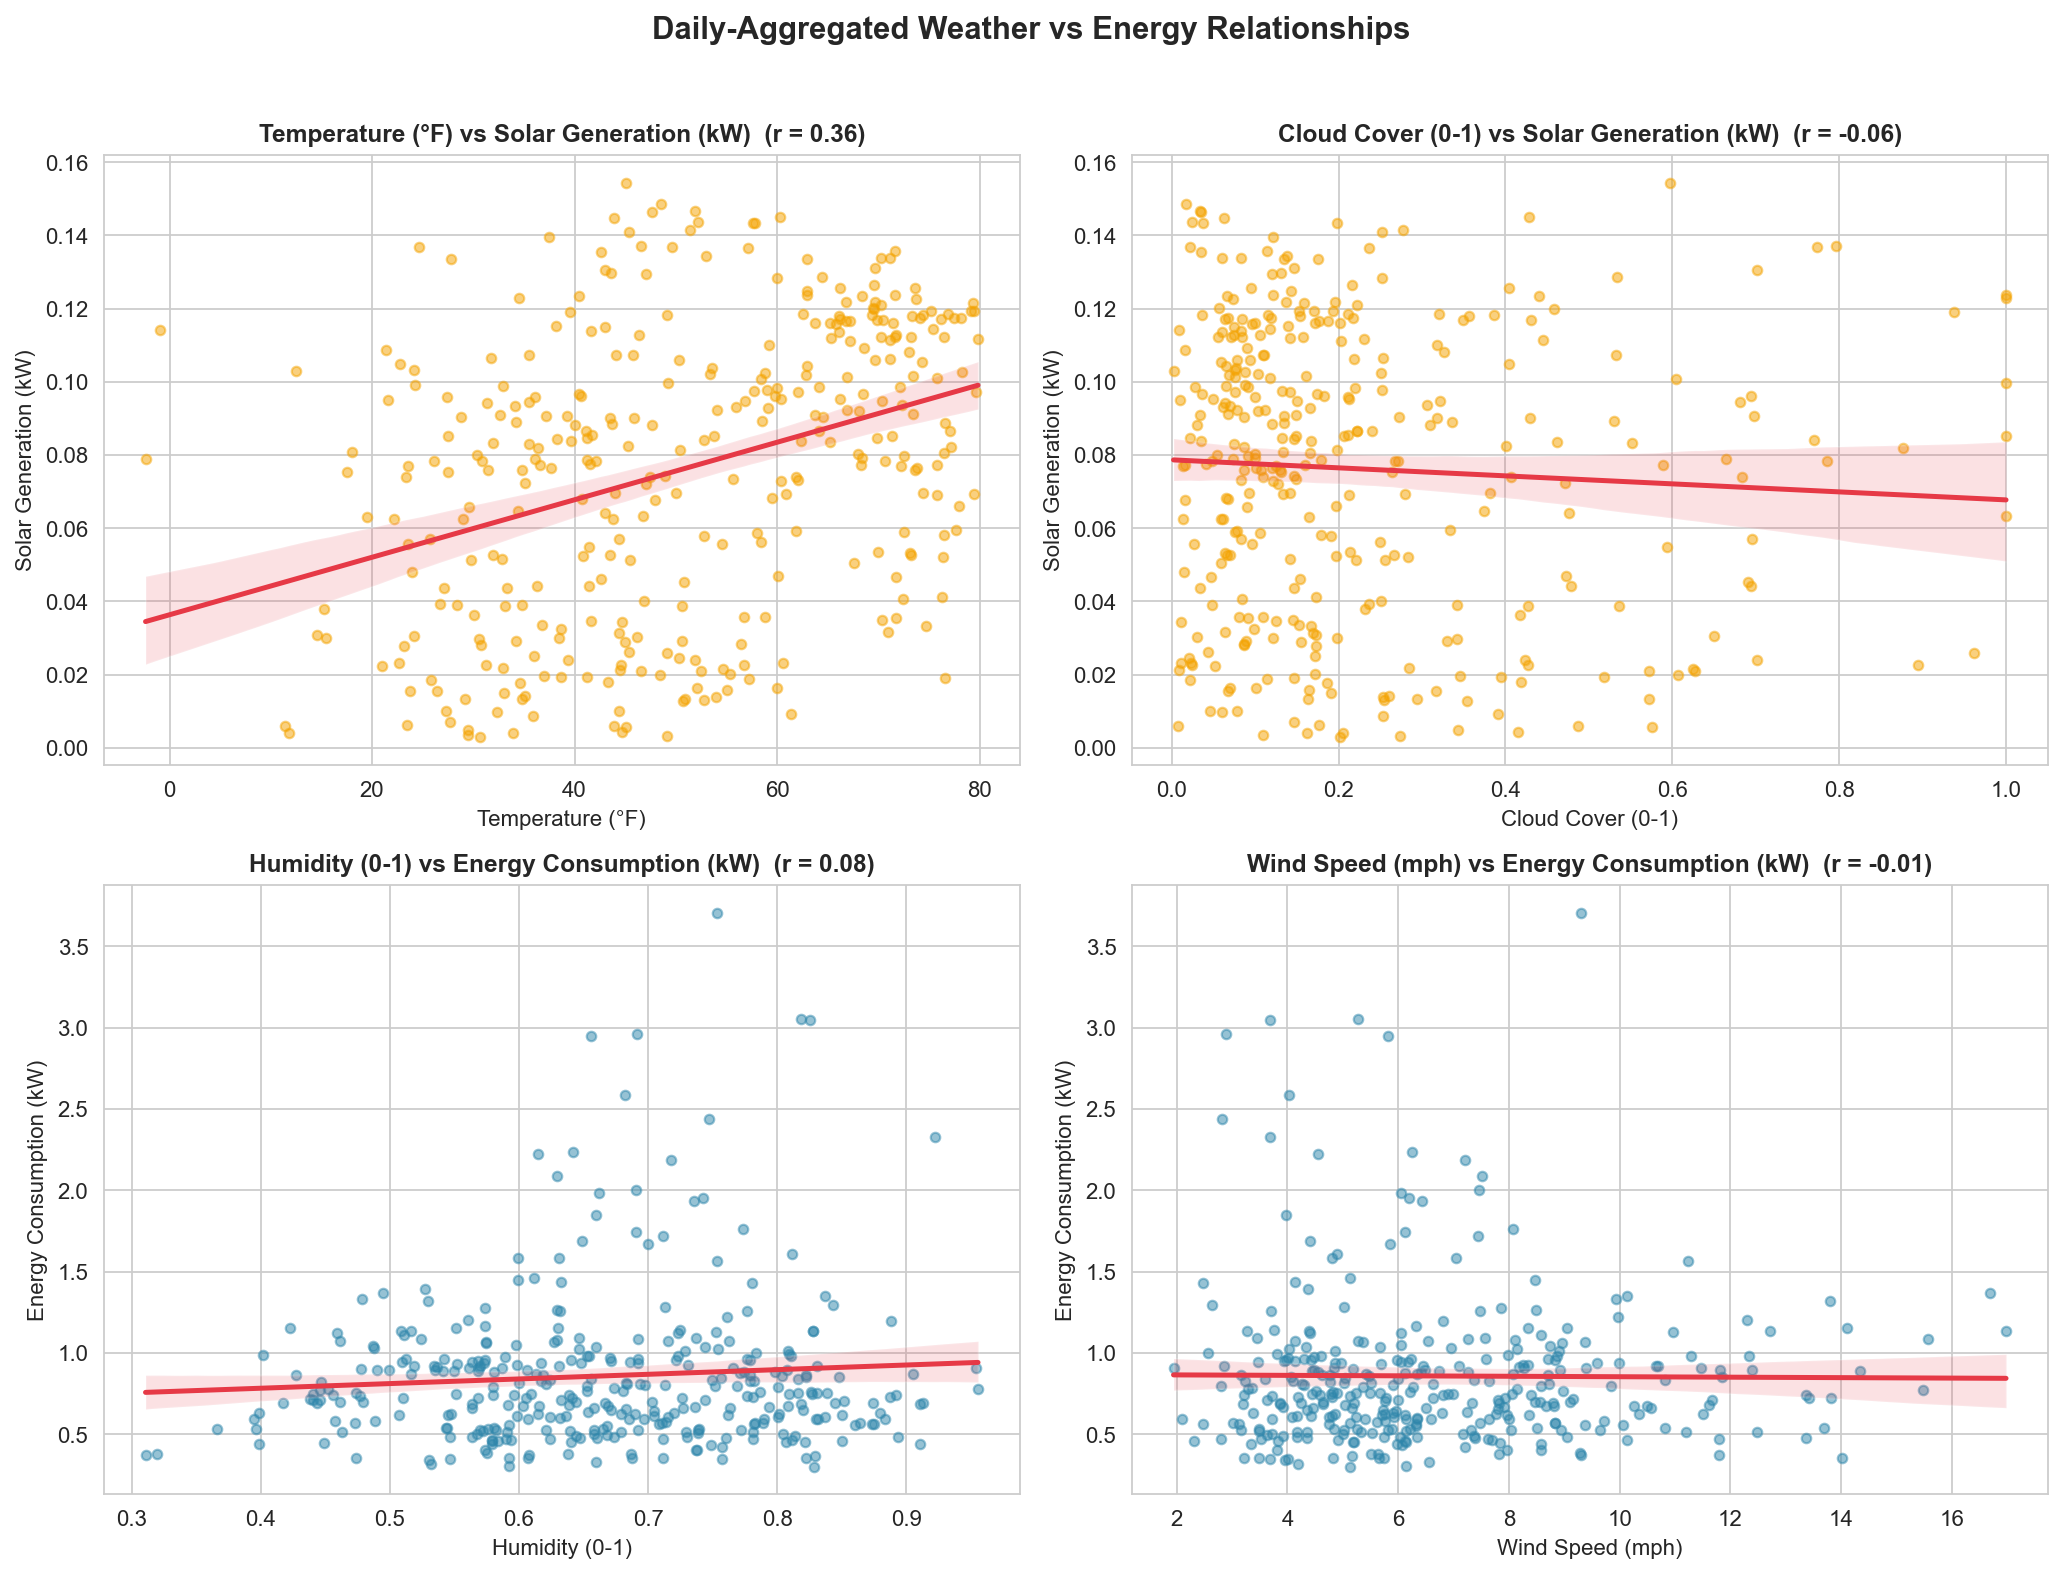
\includegraphics[width=0.95\textwidth]{figs/chart5_weather_scatter.png}
\caption{Weather versus energy and solar generation, with regression fits.}\label{fig:weather}
\end{figure}

\subsection{Temporal Usage Patterns}
Examining consumption by hour of day (Figure~\ref{fig:hourly}) and by month (Figure~\ref{fig:monthly}) reveals clear daily and seasonal rhythms that are only interpretable after the time-axis correction. Hourly demand exhibits characteristic morning and evening structure, while monthly aggregates reflect heating-driven seasonality. Figure~\ref{fig:anomaly} overlays the proxy-labelled anomalies on the consumption series, showing that flagged events cluster around the high-consumption tail rather than being uniformly distributed in time.

\begin{figure}[h]
\centering
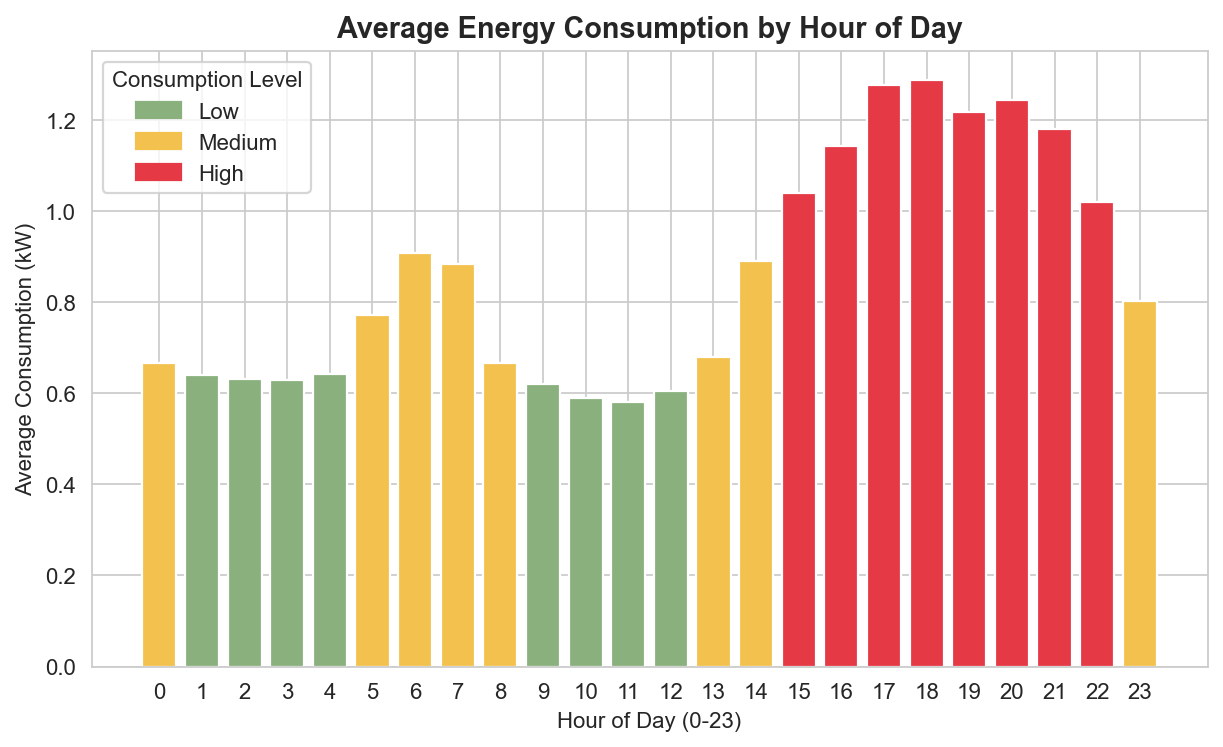
\includegraphics[width=0.85\textwidth]{figs/chart8_hourly_consumption.png}
\caption{Mean consumption by hour of day.}\label{fig:hourly}
\end{figure}

\begin{figure}[h]
\centering
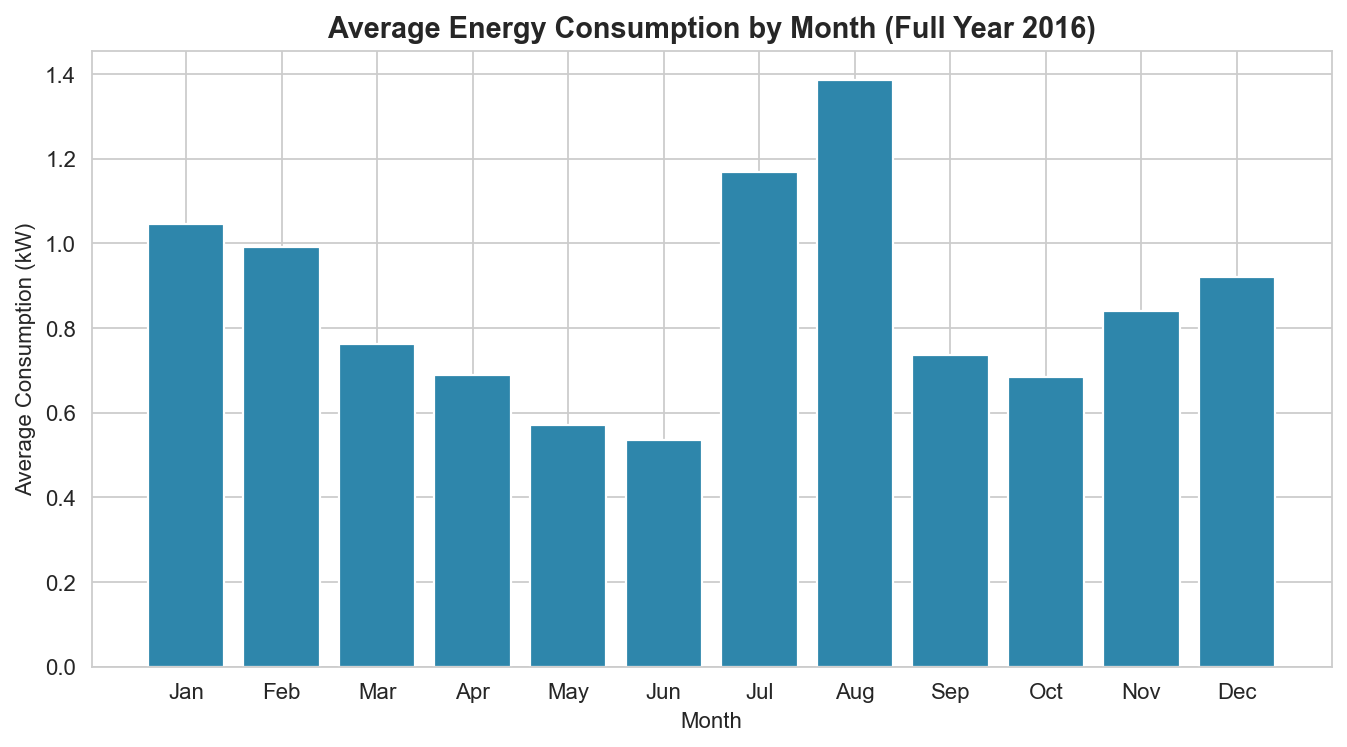
\includegraphics[width=0.75\textwidth]{figs/chart14_monthly_consumption.png}
\caption{Mean consumption by month.}\label{fig:monthly}
\end{figure}

\begin{figure}[h]
\centering
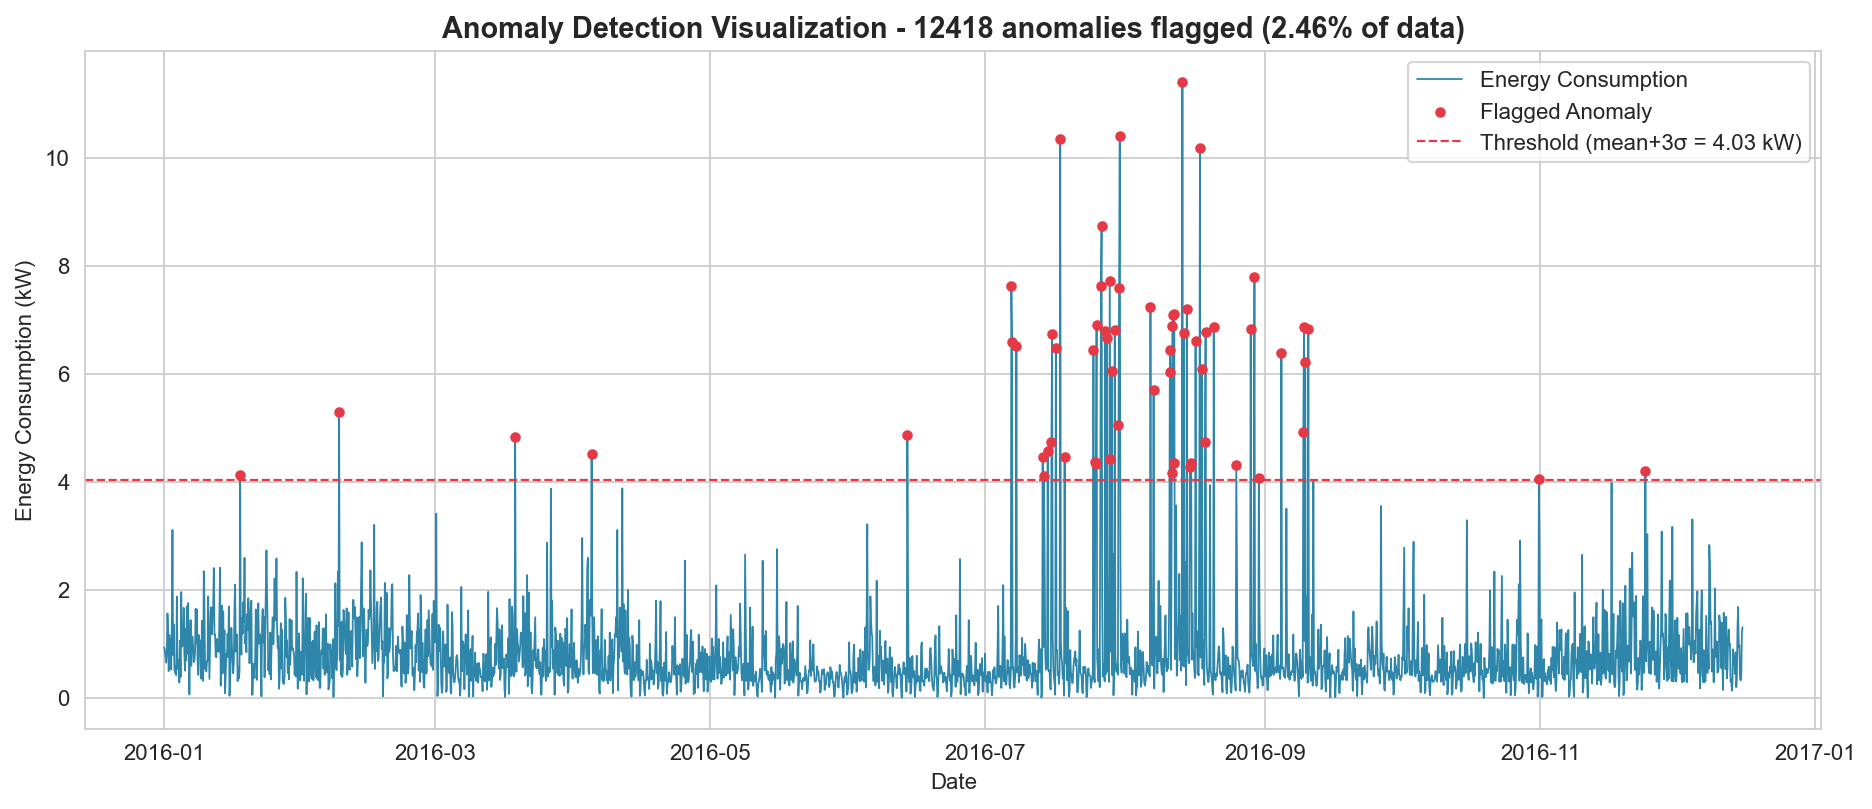
\includegraphics[width=\textwidth]{figs/chart12_anomaly_timeseries.png}
\caption{Consumption time-series with proxy-labelled anomalies marked.}\label{fig:anomaly}
\end{figure}

%%==================================%%
\section{Methodology}\label{sec:method}

\subsection{Anomaly Label Construction}
The HomeC dataset provides no ground-truth anomaly annotations. We therefore construct a transparent statistical proxy label on whole-house consumption:
\begin{equation}
\text{anomaly}_i = \mathbb{1}\!\left[\, \texttt{use}_i > \mu + k\,\sigma \,\right], \qquad k = 3,
\end{equation}
where $\mu$ and $\sigma$ are the mean and standard deviation of \texttt{use [kW]}. With $k=3$ the threshold is $4.03$ kW, producing 12{,}418 positive instances, an anomaly rate of 2.46\%. This rate falls in a reasonable range for rare-event detection and yields enough positives to train and evaluate classifiers meaningfully. We emphasise that this is a proxy, not a behavioural ground truth: the models learn to recover a threshold rule that we ourselves imposed, so the reported scores measure recoverability of that rule rather than detection of operationally confirmed faults. This limitation is revisited in Section~\ref{sec:conclusion}.

\subsection{Feature Engineering}
From the corrected time axis we derive \texttt{hour}, \texttt{dayofweek}, \texttt{month}, \texttt{is\_weekend}, \texttt{season}, and a coarse \texttt{time\_period} indicator. Appliance circuits with related semantics are grouped (the two Furnace circuits and the Kitchen circuits), and a \texttt{total\_appliance} aggregate is added. The two categorical weather fields (\texttt{icon}, \texttt{summary}) are one-hot encoded. Critically, \texttt{use [kW]} is excluded from the feature set: since the label is derived directly from it, retaining it would constitute target leakage and inflate scores toward a trivial $F1 \approx 1$.

\subsection{Pipeline and Imbalance Handling}
Data are split into training and test partitions (80/20) with stratification on the label to preserve the class ratio. Standardisation is fit on the training partition only and then applied to the test partition, preventing information from the test set leaking into preprocessing. To address class imbalance, SMOTE oversampling is applied to the training partition only. The final deliverable is a scikit-learn \texttt{Pipeline} bundling the scaler and the best estimator, so that the downstream application can call a single \texttt{predict} method without re-implementing preprocessing. The end-to-end architecture is shown in Figure~\ref{fig:arch}.

\begin{figure}[h]
\centering
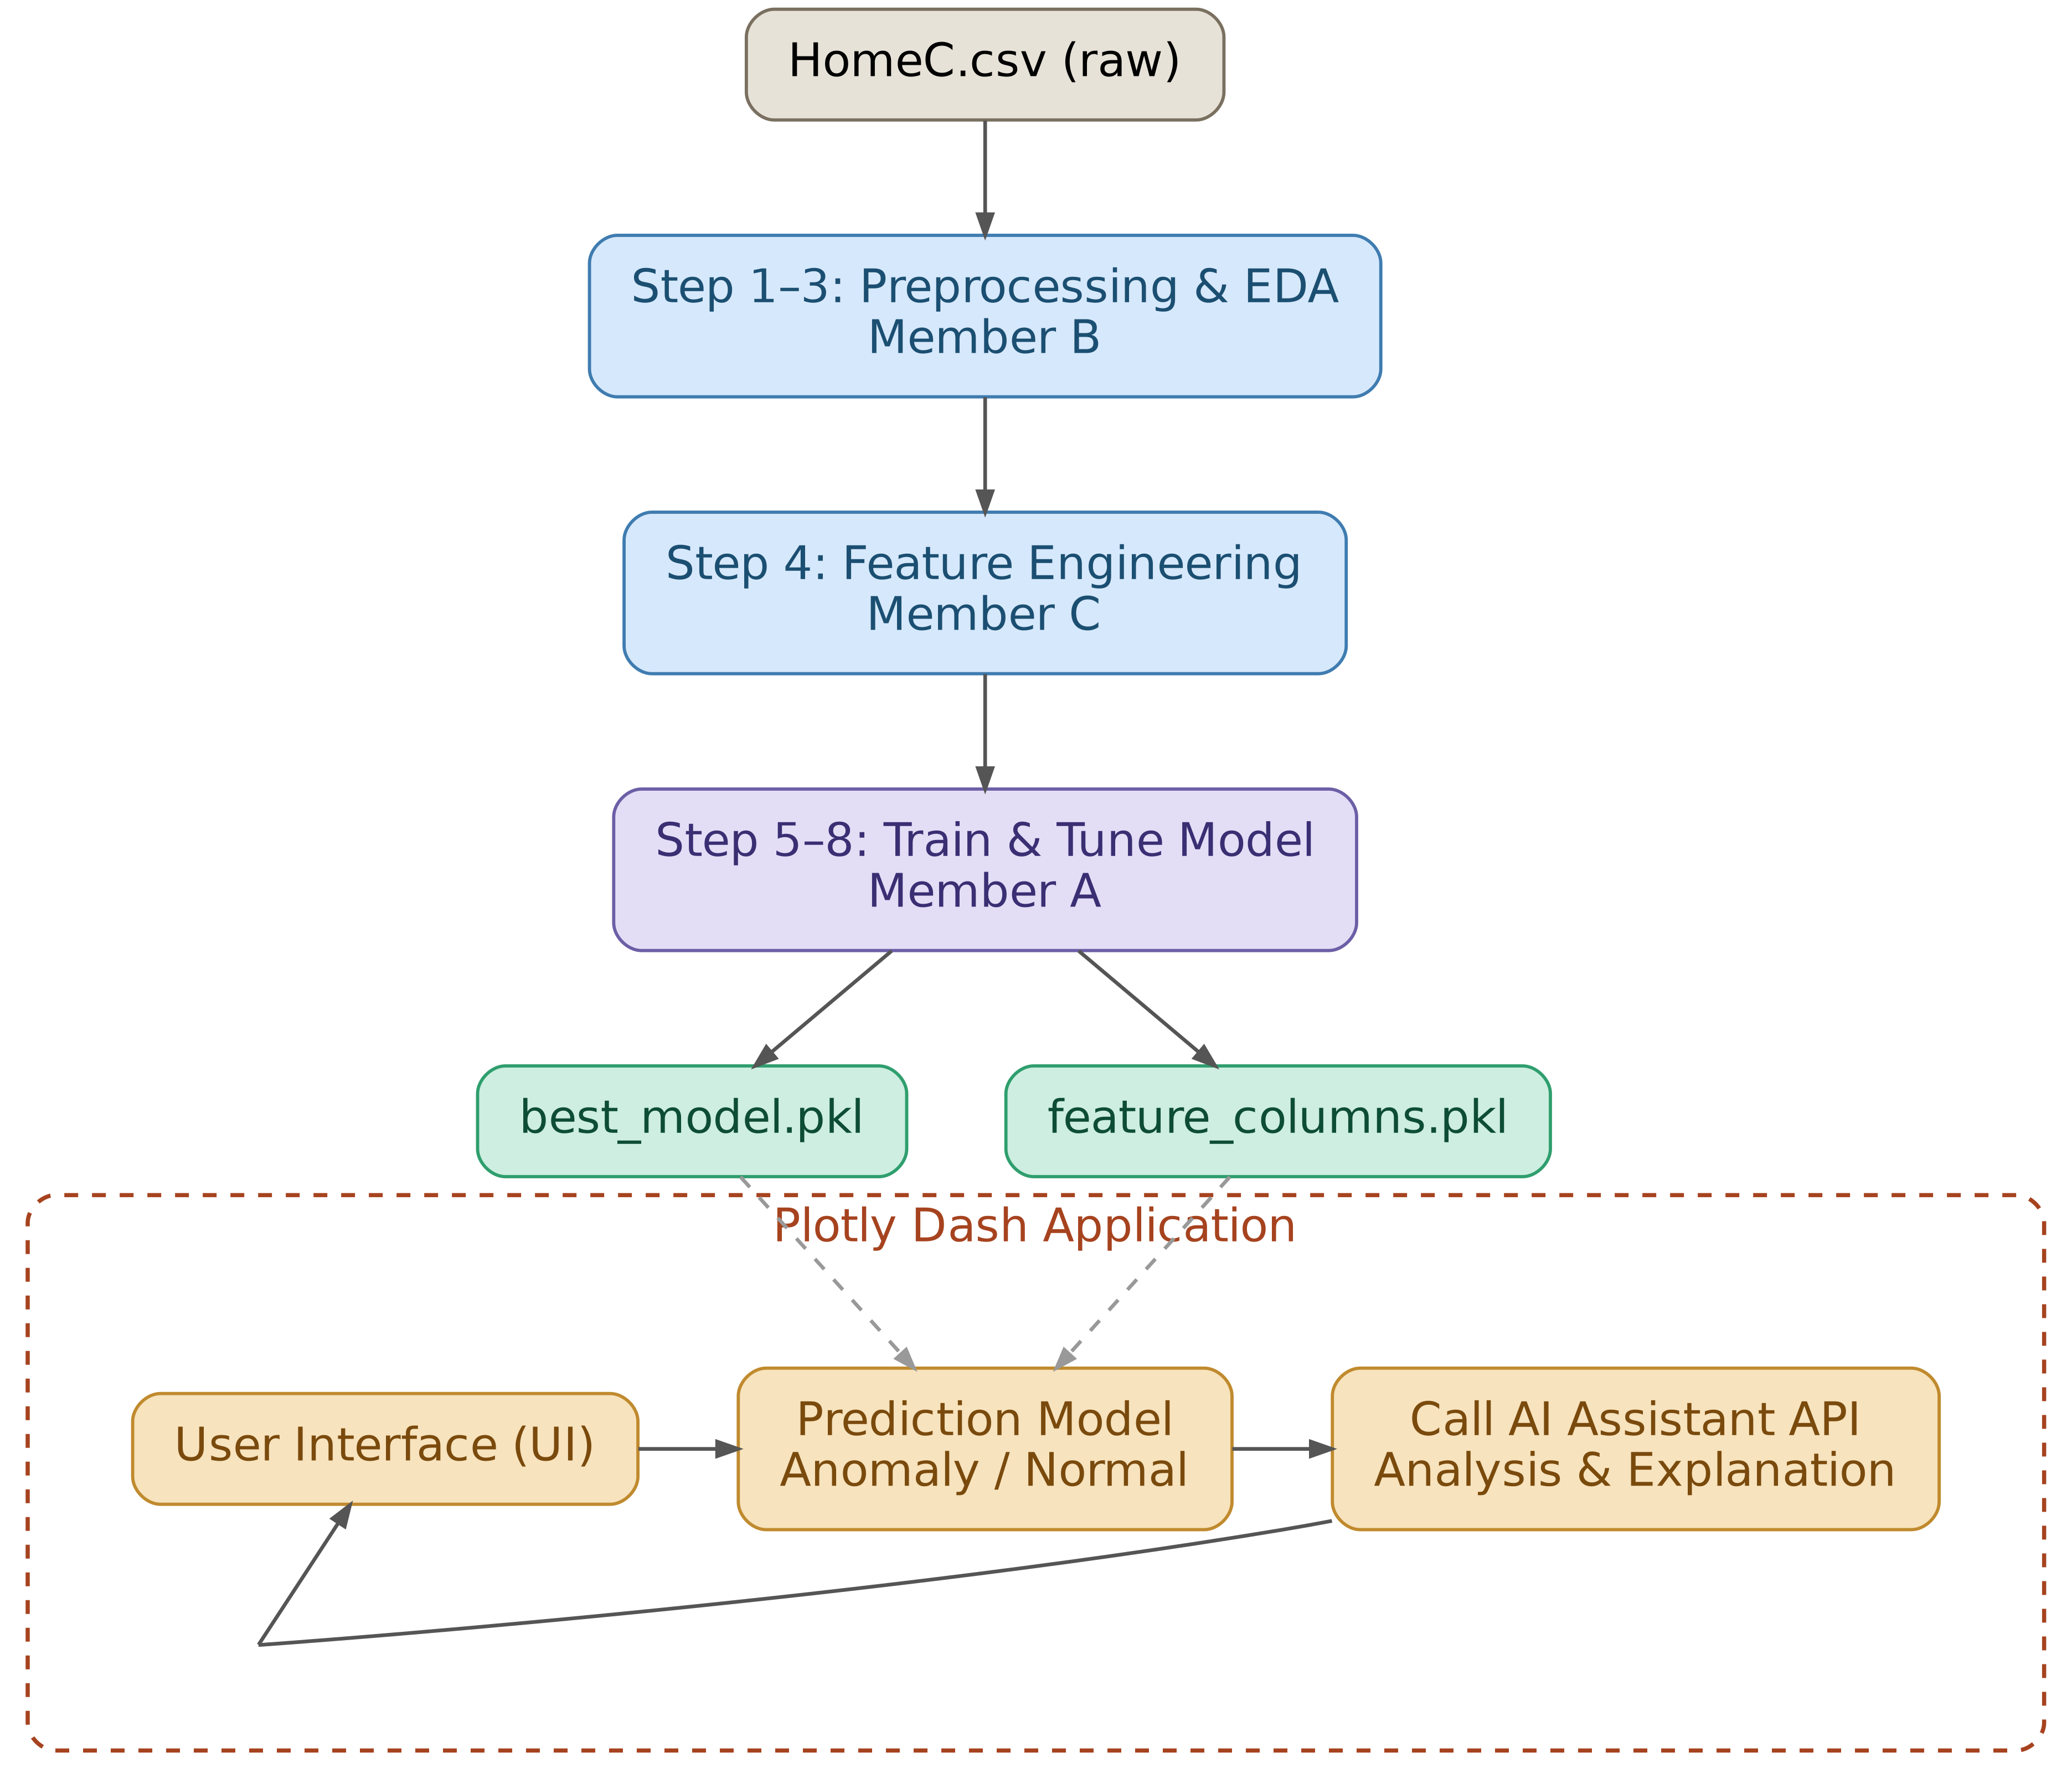
\includegraphics[width=0.9\textwidth]{figs/architecture.png}
\caption{End-to-end pipeline: preprocessing and EDA, feature engineering, model training, and the interactive dashboard.}\label{fig:arch}
\end{figure}

\subsection{Models and Evaluation Metrics}
Five models spanning linear, ensemble, and unsupervised families are benchmarked: Logistic Regression, Random Forest, XGBoost, LightGBM, and Isolation Forest. Kernel SVM variants are excluded because their cost is prohibitive on a half-million-row dataset. Hyper-parameter tuning for the leading tree-based model uses randomised search with stratified $k$-fold cross-validation over a small grid (number of estimators, tree depth/leaves, and learning rate).

Given the strong class imbalance, accuracy is an inadequate metric: a degenerate classifier predicting "normal" everywhere would score near 98\%. We therefore evaluate primarily with the F1-score, the harmonic mean of precision and recall,
\begin{equation}
F1 = \frac{2 \cdot \text{Precision} \cdot \text{Recall}}{\text{Precision} + \text{Recall}},
\end{equation}
and with AUC-ROC, which measures threshold-independent ranking ability and is well suited to detection tasks where the operating threshold may vary.

%%==================================%%
\section{Results and Evaluation}\label{sec:eval}

Table~\ref{tab:results} reports test-set performance for all five models. Random Forest is the strongest detector, with an F1 of 0.941 and near-perfect AUC, narrowly ahead of XGBoost (F1 = 0.933) and LightGBM (F1 = 0.896). The three tree-ensemble methods clearly dominate the linear and unsupervised baselines: Logistic Regression attains high recall but poor precision (F1 = 0.384), reflecting difficulty separating the classes with a linear boundary, while Isolation Forest performs worst (F1 = 0.094), indicating that a purely unsupervised partitioning does not align well with the threshold-based proxy label.

\begin{table}[h]
\caption{Test-set performance of the five benchmarked models}\label{tab:results}
\begin{tabular}{@{}lrrrr@{}}
\toprule
Model & F1 & AUC & Precision & Recall \\
\midrule
\textbf{Random Forest} & \textbf{0.9412} & \textbf{0.9996} & \textbf{0.9260} & \textbf{0.9569} \\
XGBoost            & 0.9331 & 0.9994 & 0.9178 & 0.9489 \\
LightGBM           & 0.8964 & 0.9990 & 0.8450 & 0.9545 \\
Logistic Regression & 0.3838 & 0.9706 & 0.2419 & 0.9279 \\
Isolation Forest    & 0.0945 & 0.7694 & 0.0970 & 0.0922 \\
\botrule
\end{tabular}
\footnotetext{Best result per column in bold. F1, Precision, and Recall are reported for the positive (anomaly) class.}
\end{table}

The very high AUC values for the tree ensembles indicate that, once expressive non-linear interactions among appliance and time features are available, the proxy-labelled anomalies are highly separable. The gap between Logistic Regression's strong recall and weak precision is consistent with a decision surface that captures most positives but admits many false alarms---behaviour that F1 penalises and accuracy would have masked. These results answer RQ2: among the methods tested, Random Forest provides the best balance of precision and recall on this dataset.

%%==================================%%
\section{Application and Deployment}\label{sec:app}

The trained pipeline is integrated into an interactive dashboard built with Plotly and Dash. The dashboard reads precomputed summary artefacts so that displayed figures are derived from data rather than hard-coded. It presents four key-performance-indicator cards (total energy, average power, peak consumption, and number of anomalies), an alert panel that lists the most prominent abnormal periods together with the appliance contributing most at each time, ten interactive charts mirroring the exploratory analysis, and a recommendation panel that translates the findings---dominant appliances, peak hours, and weather correlations---into actionable energy-saving suggestions. A prediction interface lets a user enter operating conditions and receive an anomaly classification, accompanied by a natural-language explanation generated through an AI service when available and a deterministic rule-based explanation otherwise.

%%==================================%%
\section{Conclusion and Future Work}\label{sec:conclusion}

This study presented an end-to-end analysis of anomaly detection on the HomeC smart-home energy dataset. After correcting a time-axis defect that had previously collapsed the record into a few days, we conducted a full exploratory analysis, engineered time- and appliance-based features, and benchmarked five models under a leakage-controlled pipeline. Returning to the research questions: appliance usage---heating circuits above all, at roughly 56\% of metered appliance energy---is the dominant factor associated with abnormal consumption (RQ1); Random Forest is the best-performing detector, at F1 = 0.941 and AUC = 0.9996 (RQ2); and weather correlates meaningfully with solar generation but only weakly with raw household demand (RQ3).

Several limitations frame these results. The anomaly label is a statistical proxy derived from a $\mu + 3\sigma$ threshold rather than operationally confirmed faults, so the high scores reflect the recoverability of an imposed rule, not validated fault detection. The analysis also covers a single household over one year, which constrains generalisation. Future work should pursue externally validated labels (for example, maintenance records or expert annotation), evaluate genuinely temporal models that exploit sequential dependence, and test transferability across multiple homes. Incorporating richer semantic and contextual features would further strengthen the link between detected anomalies and their real-world causes.

\backmatter

\bmhead{Acknowledgements}
The authors thank the course instructors and mentors for their guidance throughout the project.

\section*{Declarations}
\begin{itemize}
\item \textbf{Data availability.} The HomeC dataset (Smart Home Dataset with Weather Information) is publicly available on Kaggle.
\item \textbf{Competing interests.} The authors declare no competing interests.
\end{itemize}

\end{document}
